%% WSDM 2027 camera-ready version.
%% Main text is targeted to nine pages; Ethical Considerations and references follow.
\documentclass[sigconf]{acmart}

\usepackage{booktabs}
\usepackage{graphicx}
\usepackage{amsmath}
\usepackage{array}
\usepackage{tabularx}
\usepackage{microtype}
\usepackage{xcolor}
\usepackage{pifont}

\copyrightyear{2027}
\acmYear{2027}
\setcopyright{cc}
\setcctype{by}
\acmConference[WSDM '27]{Proceedings of the Twentieth ACM International Conference on Web Search and Data Mining}{February 15--19, 2027}{Hong Kong, Hong Kong}
\acmBooktitle{Proceedings of the Twentieth ACM International Conference on Web Search and Data Mining (WSDM '27), February 15--19, 2027, Hong Kong, Hong Kong}
\acmDOI{10.1145/3862322.3863501}
\acmISBN{979-8-4007-3117-4/2027/02}

\AtBeginDocument{\providecommand\BibTeX{{Bib\TeX}}}
\newcommand{\cpoison}{\textsc{Poisoned}}
\newcommand{\cclean}{\textsc{Clean}}
\newcommand{\cmixed}{\textsc{Mixed}}
\newcommand{\cinsuf}{\textsc{Insufficient}}
\newcommand{\CGrV}{CGrV}
\setlength{\emergencystretch}{3em}
% TeX hyphenates neither component of a word that already contains an explicit
% hyphen, and "verbalized-probability" is too wide to end a nine-point line, so
% its break points are supplied by hand.
\newcommand{\vprob}{ver\-bal\-ized-prob\-a\-bil\-ity}


\newcommand{\uc}{U_c}
\newcommand{\ac}{a_C}
\newcommand{\ar}{a_R}
\newcommand{\ap}{a_P}


\begin{document}

\title[Attributing Learned Arbitration under Misleading Retrieval]
{Attributing the Value of Learned Source Arbitration under Misleading Retrieval:
A Cross-Fitted Comparator Audit}

%% TODO(camera-ready): replace every placeholder below. Names, order,
%% affiliations, and e-mail addresses must match CMT and the ACM rights
%% form exactly.
\author{Minsu Oh}
\affiliation{%
  \institution{Jeju National University}
  \city{Jeju}
  \country{Republic of Korea}}
\email{dhals0517@stu.jejunu.ac.kr}
\orcid{0009-0002-8093-5967}

\author{Chanjun Park}
\authornote{Corresponding authors.}
\affiliation{%
  \institution{Soongsil University}
  \city{Seoul}
  \country{Republic of Korea}}
\email{chanjun.park@ssu.ac.kr}
\orcid{0000-0002-7200-9632}

\author{Yeo Chan Yoon}
\authornotemark[1]
\affiliation{%
  \institution{Jeju National University}
  \city{Jeju}
  \country{Republic of Korea}}
\email{ycyoon@jejunu.ac.kr}
\orcid{0000-0002-5573-8964}

\begin{abstract}
Retrieval-augmented generation (RAG) can fail when retrieved passages
contain false answers. Across three benchmarks, false-answer contexts
pass sufficiency checks more often than insufficient ones; an LLM
instructed to follow the context repeats the false answer in $74\%$ of
poisoned ClashEval cases. Recent methods use selectors that choose which
answer source to trust. Evaluations against fixed single-source baselines can mix
two effects: using alternative answer sources and learning how to choose
among them. We introduce a cross-fitted comparator audit that freezes
answers from the supplied context, independent retrieval, and model
knowledge, then compares instance-specific methods with deterministic
agreement and fallback rules. Each method family chooses what to deploy
on one question fold and is evaluated on the other, then the fold roles
reverse. On $400$ cases from four datasets not used for fitting,
instance-specific methods improve over the context-only rule, but are
generally no better than, and often worse than, deterministic rules
selected on the same held-out questions. 
The same pattern persists with two additional LLMs, across three
additional collections after local comparator selection, and on
low-popularity factual questions.
Gains over a fixed single-source baseline can therefore reflect access
to a stronger alternative answer source rather than instance-specific
learning, so learned arbitration should be evaluated against comparators
given the same selection opportunity.
\end{abstract}

%% TODO(camera-ready): confirm both concept IDs against the code generated
%% at https://dl.acm.org/ccs before submission.
\begin{CCSXML}
<ccs2012>
   <concept>
       <concept_id>10002951.10003317</concept_id>
       <concept_desc>Information systems~Information retrieval</concept_desc>
       <concept_significance>500</concept_significance>
       </concept>
   <concept>
       <concept_id>10010147.10010178.10010179.10010182</concept_id>
       <concept_desc>Computing methodologies~Natural language generation</concept_desc>
       <concept_significance>300</concept_significance>
       </concept>
 </ccs2012>
\end{CCSXML}

\ccsdesc[500]{Information systems~Information retrieval}
\ccsdesc[300]{Computing methodologies~Natural language generation}
\keywords{retrieval augmented generation, source arbitration, answer selection, comparator evaluation, selective prediction}
\maketitle

\section{Introduction}\label{sec:intro}
\begin{figure}[t]
  \centering
  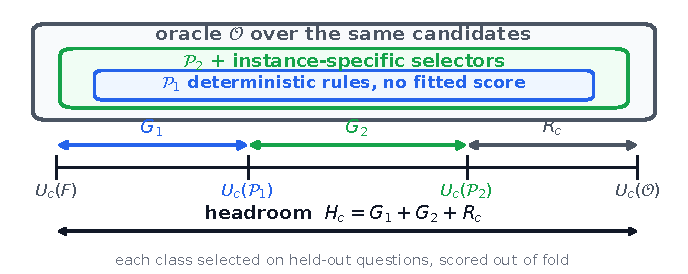
\includegraphics[width=\columnwidth]{figures/fig_protocol.pdf}
  \Description{A comparison from a context-only baseline to deterministic multi-source rules, a broader instance-specific class, and an oracle over the same candidate answers.}
  \caption{Cross-fitted comparator audit. All methods act on the same
  fixed candidate answers. The deterministic class $\mathcal{P}_1$ and
  the broader instance-specific class $\mathcal{P}_2$ each select one
  member on one question fold and are evaluated on the other, then the
  folds reverse. $G_1$ is the gain from deterministic multi-source
  selection, $G_2$ the additional instance-specific gain, and $R_c$ the
  remaining gap to the oracle.}
  \label{fig:protocol}
\end{figure}

Retrieval-augmented generation conditions its output on retrieved
evidence~\cite{lewis2020rag}. When that evidence is misleading, a
passage may contain enough information to derive an answer without
being credible. Across three conflict benchmarks, contexts asserting a
false answer pass sufficiency screening more often than insufficient
contexts. On ClashEval~\cite{wu2024clasheval}, a large language model
(LLM) instructed to follow the supplied context repeats the false
answer in $74\%$ of poisoned cases.

Recent methods use reliability estimates, conflict-aware prompting, or
likelihood margins to decide whether retrieved evidence or model
knowledge should guide an answer~\cite{zhu2026saber,choi2025care,xu2026trustmargin}.
An answer selector chooses which candidate answer to return for a
question, or abstains. Prior work commonly reports performance against single-source baselines,
including closed-book parametric answers and context-conditioned RAG
answers. An arbitration method has access to both sources, so an
improvement over either fixed baseline can combine two effects: access
to the alternative source and question-specific selection between
sources. Isolating the value added by arbitration therefore requires a
comparator with access to the same candidate answers and the same
opportunity for policy selection.

We introduce a cross-fitted comparator audit to separate these effects.
We use a fixed LLM, which we call the reader, to generate three answers
independently from the supplied context, a separately retrieved
reference corpus, and the model's own knowledge. The answers are then
fixed. We compare $23$ deterministic agreement and fallback rules with
a broader family of instance-specific methods, including learned,
LLM-based, likelihood-based, and structured selectors. 
Each family selects one member on one question fold and is evaluated on the other,
then the fold roles reverse. The audit therefore estimates the
incremental value of instance-specific methods when both families may
use labelled target questions for selection; it does not determine what
to deploy on a target without labels.

On a $400$-case evaluation from four collections not used for fitting,
gradient boosting and the LLM-based selector outperform the context-only
rule, but once deterministic rules are selected on the same held-out
target questions, the instance-specific methods are generally no better
and are often worse. 
On a separate $300$-case evaluation from three additional collections,
the LLM-based selector outperforms a deterministic rule selected on the
preceding $400$-case evaluation and carried over unchanged. The same
advantage is not observed when the deterministic family is instead
allowed to select a rule using questions from the $300$-case evaluation
itself. No corresponding interval excludes zero with two additional readers or
on factual questions involving either high- or low-popularity entities. 
When retrieval is known to contain an accepted
answer and the retrieval-based answer becomes stronger than the model
answer, the selected deterministic rule shifts toward retrieval without
an additional instance-specific gain.

Comparisons with prior methods support the same attribution. A
frozen-candidate adaptation of TrustMargin enters the instance-specific
family but changes no selected method or stage difference. On its native
candidate set, our reimplementation of SABER does not outperform a
deterministic two-source
comparator selected by the same cross-fit protocol. These comparisons
do not imply that learned arbitration is unnecessary. They show that
its incremental value must be measured against simpler comparators
given the same candidate answers and the same data for policy selection.
Figure~\ref{fig:pipeline} summarizes the evaluation pipeline. We release
code and reproducibility artifacts with a driver for the headline
results.\footnote{\url{https://github.com/ycyoon/misleading-retrieval-stagewise-release}}

\section{Related Work}\label{sec:related}

\paragraph{Misleading retrieval and knowledge conflict.}
Retrieval-augmented generation can fail when retrieved evidence is missing, conflicting, or misleading, as studied by ClashEval~\cite{wu2024clasheval}, RAMDocs~\cite{wang2025ramdocs}, RAGuard~\cite{raguard2024}, the Retrieval-Augmented Generation Benchmark (RGB)~\cite{chen2024rgb}, WhoQA~\cite{pham2024whoqa}, NeoQA~\cite{glockner2025neoqa}, and MAGIC~\cite{lee2025magic}, and by work on retrieval corruption as an adversarial attack~\cite{zou2025poisonedrag,xiang2026robustrag,tan2025revprag}. A language model may follow retrieved evidence even when it conflicts with a correct answer or with its internal knowledge. We use several of these collections to measure this failure and to fit the answer-selection methods, keeping all variants of a question in the same split, and perform the main selection comparison on separate collections not used for fitting.

\paragraph{Selective prediction and calibration.}
Selective QA studies when a model should answer or abstain. Confidence
can degrade under domain shift~\cite{kamath2020selective}, and
generative QA probabilities can be poorly calibrated to answer
correctness~\cite{jiang2021calibration}. Our setting additionally
chooses among multiple frozen answer sources, so a gain can reflect
either better confidence estimation or access to a stronger source.

\paragraph{Verification, source arbitration, and abstention.}
One line of work decides whether retrieved evidence should be used at
all. Sufficient Context tests whether retrieved evidence contains
enough information to answer a question~\cite{joren2024sufficient},
while SURE-RAG determines whether evidence supports, refutes, or is
insufficient for a candidate answer~\cite{qiu2026surerag}. Such
judgments address answerability or support, but support does not
establish factual credibility when the retrieved passage itself is
misleading.

Other methods change retrieval, source assessment, reasoning, or
generation under unreliable evidence. Astute RAG~\cite{wang2024astute},
FaithfulRAG~\cite{zhang2025faithfulrag},
Micro-Act~\cite{huo2025microact}, RA-RAG~\cite{rarag2024},
CRAG~\cite{yan2024crag}, Self-RAG~\cite{asai2024selfrag}, and
CrAM~\cite{deng2024cram} combine internal knowledge, retrieval
correction, self-reflection, or modified generation. These methods
address how to produce a better answer under imperfect evidence, but
their end-to-end gains can combine the benefit of using alternative
information sources with the benefit of question-specific arbitration.
Because these methods change how candidates are produced, they fall
outside our frozen-candidate abstraction; we do not evaluate them, and
our conclusions do not extend to them.

Closer to our setting, SABER estimates the reliability of contextual
and parametric answer paths~\cite{zhu2026saber}, CARE uses
conflict-aware soft prompting when retrieved evidence and model
knowledge disagree~\cite{choi2025care}, and TrustMargin selects between
closed-book and retrieval-augmented answers using likelihood
margins~\cite{xu2026trustmargin}. We compare with these prior methods
where their decision process can be matched to our candidate space, and
report native end-to-end results separately when a method changes
candidate generation. The central evaluation question is not whether a
more complex method can beat a context-only default, but how much of
that gain remains after a deterministic multi-source comparator receives
the same candidate answers and the same held-out questions for policy selection.

\begin{figure*}[t]
  \centering
  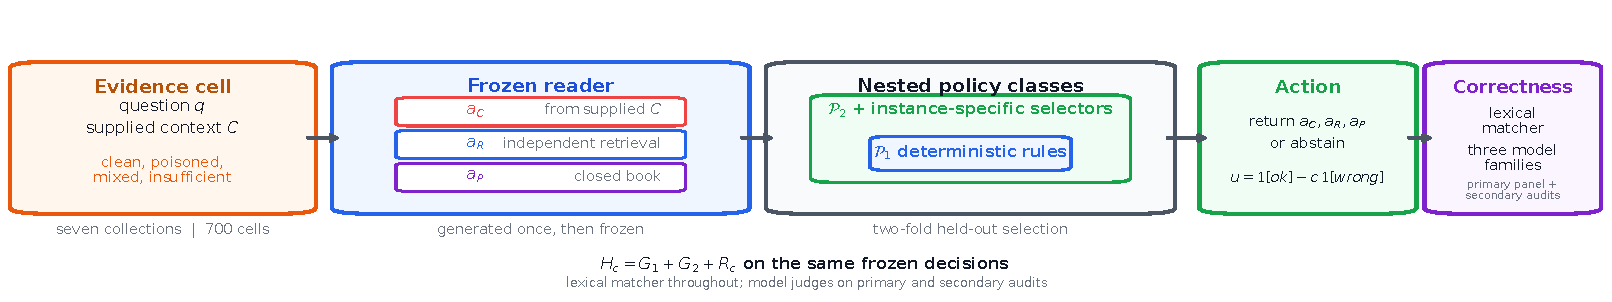
\includegraphics[width=\textwidth]{figures/fig_pipeline.pdf}
  \Description{A left-to-right pipeline in which a fixed language model generates context, reference-retrieval, and model-knowledge answers; deterministic and instance-specific methods choose one answer or abstain; and lexical and semantic criteria judge correctness.}
  \caption{Evaluation pipeline. Three candidate answers are generated
  independently and then fixed. Deterministic and instance-specific
  methods act on the same candidate set and either return one candidate
  or abstain. The lexical matcher is the common correctness criterion;
  model-based judgments provide semantic sensitivity analyses.}
  \label{fig:pipeline}
\end{figure*}


\section{Problem and Evaluation Protocol}
\label{sec:setup}

\subsection{Evidence conditions and independent candidates}

A question can appear with a \cclean{} context that supports an
accepted answer, a \cpoison{} context that states a false answer, a
\cmixed{} context that contains both, or an \cinsuf{} context that
does not answer it. These labels describe the evidence presented to
the reader and are used only for diagnosis, never as selector
features. A question paired with one supplied context forms one
evaluation cell.

For the sufficiency diagnostic, let $S=1$ denote a passing judgment. We
report $\Delta_{\mathrm{suff}}
=\Pr(S=1\mid\cpoison)-\Pr(S=1\mid\cinsuf)$; positive values mean that
misleading contexts pass more often than insufficient ones.

For question $q$, supplied context $C$, and independently retrieved
reference passages $R$, a frozen reader $G$ produces
\begin{equation}
  \ac=G(q,C), \qquad
  \ar=G(q,R), \qquad
  \ap=G(q).
  \label{eq:candidates}
\end{equation}
Each candidate is generated independently, without access to the
answers produced from the other sources. The reference passages come
from the Wikipedia collection released with Dense Passage
Retrieval~\cite{karpukhin2020dpr}, encoded with the
BGE-base-en-v1.5 model~\cite{xiao2023bge} and searched with
FAISS~\cite{johnson2019faiss}. The main reader is
Qwen2.5-72B-Instruct~\cite{qwen2024qwen25}, used with temperature
zero. Section~\ref{sec:res-ladder} repeats the full comparator audit
with Llama-3.1-70B-Instruct and Llama-3.1-8B-Instruct
~\cite{dubey2024llama3}, each on its own candidate set over the
same $400$ primary-panel cells.

For answer-selection experiments on evaluation collections not used to
fit the learned selectors, a candidate is \emph{available} when the generation pipeline extracts a nonempty
answer and the answer is not one of the frozen refusal forms
\emph{I don't know}, \emph{I dont know}, \emph{unknown}, or
\emph{n/a} after case folding.

\subsection{Verification, selection, and decision score}

We evaluate two decision problems. In \emph{verification}, the system
either returns the answer generated from the supplied context, $\ac$,
or abstains. In \emph{answer selection}, the system may return $\ac$,
the independently retrieved answer $\ar$, the closed-book parametric
answer $\ap$, or abstain.

We summarize each decision with a \emph{decision score}, denoted by
$U_c$. A correct answer receives $+1$, a wrong answer receives $-c$,
and abstention receives $0$:
\begin{equation}
  \uc =
  \mathbf{1}[\text{correct return}]
  - c\,\mathbf{1}[\text{wrong return}].
  \label{eq:utility}
\end{equation}
Here $c$ controls how strongly wrong answers are penalized. We evaluate
$c\in\{0.5,1,2,4\}$; larger values favour more conservative
policies. The decision score does not use the evidence-condition label
and gives the same credit to a correct answer recovered from a poisoned
context.

\subsection{Cross-fitted comparator attribution}
\label{sec:attribution}

To attribute an improvement to question-specific arbitration, all
method families must act on the same candidate answers and use the same
held-out target questions to choose what to deploy. We call a decision
rule a \emph{policy}: it maps the available candidate answers to one
returned answer or to abstention. Let $F$ be the context-only policy,
which returns $\ac$ when available and otherwise abstains. Let $O$ be an
oracle over the same three candidates. It returns a correct candidate
whenever one exists and otherwise abstains. The candidate headroom is
\begin{equation}
  H_c = U_c(O)-U_c(F),
\end{equation}
the largest score improvement available from the already generated
candidates.

We compare two nested policy classes,
$\mathcal{P}_1\subset\mathcal{P}_2$.
$\mathcal{P}_1$ contains the $23$ deterministic rules in
Table~\ref{tab:det-policies}. They use candidate availability and exact
agreement between normalized answer strings, but do not fit a
question-specific score.

\begin{table}[t]
\centering
\footnotesize
\caption{The $23$ deterministic policies in $\mathcal{P}_1$.
An arrow specifies a fixed fallback order; $x,y\in
\{\ac,\ar,\ap\}$ and $x\neq y$.}
\label{tab:det-policies}
\begin{tabularx}{\columnwidth}{@{}l c X@{}}
\toprule
Type & \# & Definition \\
\midrule
Single source
& 3 & $\ac$, $\ar$, $\ap$ \\

Abstain
& 1 & always abstain \\

Two-source fallback
& 6 & all ordered rules $x\!\to\!y$ \\

Three-source fallback
& 6 & all permutations of $(\ac,\ar,\ap)$ \\

Pairwise agreement
& 3 & $\ac=\ar$, $\ac=\ap$, $\ar=\ap$ \\

Any-pair agreement
& 1 & answer when any pair agrees \\

Agreement + fallback
& 3 & any-pair$\!\to\!\ac$,
      any-pair$\!\to\!\ar$,
      any-pair$\!\to\!\ap$ \\
\midrule
Total & 23 & \\
\bottomrule
\end{tabularx}
\end{table}

The three single-source policies return $\ac$, $\ar$, or $\ap$ when
that candidate is available and otherwise abstain. A fallback policy
returns the first available answer in its listed order and abstains
when none is available. Agreement policies lowercase
answers and collapse repeated whitespace before testing exact string
equality. The any-pair policy answers when any two candidates agree;
its three fallback variants use the specified source when no pair
agrees. Exact matching defines only the deterministic rules: methods in
$\mathcal{P}_2$ may use semantic signals, and correctness is judged
separately (Section~\ref{sec:inference}).

$\mathcal{P}_2$ contains all $23$ deterministic policies plus gradient
boosting, an LLM-based candidate selector, a context-only
$p_{\mathrm{true}}$ gate, six likelihood-margin policies, a frozen-candidate
TrustMargin adaptation, and a structured relational selector, for $34$
policies in total. Section~\ref{sec:methods} defines these methods. Parameters for
the supervised methods are fitted only on the fitting pool, where the
reference answer is unavailable. The LLM-based selector,
likelihood-margin policies, and frozen TrustMargin adaptation require no
parameter fitting on that pool.

We split evaluation questions into two folds. For each cost $c$, each
policy class selects one member on one fold and is scored on the other,
then the roles reverse. We write $U_c(\mathcal{P}_k)$ for this held-out
score. The deterministic class uses the same labelled selection fold as
the broader class. It is not an ensemble: one deterministic rule is
selected for a fold and then applied unchanged to every question in the
opposite fold.
This design estimates the incremental value of expanding the policy
class when both classes may use labelled questions from the target
panel to select a member. It is therefore an attribution audit, not a
deployment comparison: it does not determine which method to deploy on
a target without labels (Section~\ref{sec:res-extension}).

The two stage differences are $G_1=U_c(\mathcal{P}_1)-U_c(F)$, the
gain from choosing a deterministic multi-source rule, and
$G_2=U_c(\mathcal{P}_2)-U_c(\mathcal{P}_1)$, the additional gain from
allowing question-specific methods;
$R_c=U_c(O)-U_c(\mathcal{P}_2)$ is the remaining oracle gap. By
definition,
\begin{equation}
  H_c = G_1+G_2+R_c.
\end{equation}
How $G_2$ is interpreted depends on the policy families, the selection
data, and the fitting distribution.
A stage difference can be negative because a broader class may select a
method that performs well on the selection fold but transfers poorly to
the other fold. Policy selection is therefore repeated inside every
bootstrap sample.

Removing the context and reference fallbacks from the
agreement-with-fallback rules yields the same selected policies and
stage differences; detailed results are released with the supplementary
artifacts. The same deterministic family is used unchanged for the
extension and both additional-reader candidate sets. Verification has
the smaller action space $\{\ac,\text{abstain}\}$ and is evaluated
separately in Section~\ref{sec:verification}.

\subsection{Data, splits, and evaluation panels}
\label{sec:data}

We pool $13{,}228$ candidate records from ClashEval, RAGuard,
RAMDocs, and RGB to fit one set of selectors across heterogeneous
conflict settings. The records contain $2{,}094$ distinct question
strings and $2{,}090$ canonical question keys after normalization
(Unicode NFKC and case folding). Records sharing a canonical
question key are assigned to the same split, preventing the same
underlying question from contributing to both policy selection and
evaluation. 
We repeat model fitting with $12$ prespecified random seeds, each using
a question-disjoint train, development, and test split of the fitting
pool. All $12$ trained runs are retained for evaluation, with each
method's decision score averaged over them; only their
development splits are used for model selection, calibration, and
threshold selection, with no run selected using external labels.

External evaluation uses $700$ cells from seven collections not used
for fitting, redistributed with SABER~\cite{zhu2026saber}.
We call the first $400$ cells the \emph{primary evaluation panel}; it
contains Natural Questions (NQ)~\cite{kwiatkowski2019nq},
TriviaQA~\cite{joshi2017triviaqa}, ConFiQA-QA~\cite{bi2025contextdpo},
and ConflictBank~\cite{su2024conflictbank}. We call the remaining
$300$ cells the \emph{extension panel}; it contains ConFiQA-MC,
ConFiQA-MR~\cite{bi2025contextdpo}, and
ConflictQA-PopQA~\cite{xie2024adaptive}.

To test whether the main result depends on parametric knowledge being
strong, we also construct head and long-tail stress panels from unused
ConflictQA-PopQA questions. The strata use the top and bottom quartiles
of the dataset's entity-popularity measure, fixed before candidate
generation. Each stratum contains $400$ cells. Normalization yields
$199$ canonical question keys in the head stratum and $200$ in the
long-tail stratum.

Before external candidate generation, we fix the question registry,
prompts, generation procedure, overlap checks, and lexical correctness
criterion. We reject any cell sharing a canonical question, question
identifier, source-passage identifier, or passage text with the fitting
data, and apply the same checks across the primary panel, extension,
and popularity stress panels. All records sharing a canonical question
key remain in the same fold. Gold answers are never included in
selector inputs, and we independently recompute the reported decision
scores from the recorded actions.

\subsection{Inference and correctness adjudication}
\label{sec:inference}

All intervals are $95\%$. For external-panel comparisons, we use a
released registry of $10{,}000$ paired bootstrap draws generated with
seed \texttt{20260807}. It preserves question-key grouping and
collection-level macro weighting, with draw identifiers shared across
methods and costs. Policy selection is repeated within each draw.

Most headline comparisons use max-$T$ simultaneous confidence
bands~\cite{westfall1993resampling} to account for multiple comparisons.
The primary family contains $15$ prespecified policy contrasts evaluated
at four costs, giving $15\times4=60$ comparisons whose intervals are
adjusted jointly. Section~\ref{sec:methods} summarizes this comparison
family. The stagewise terms in Table~\ref{tab:ladder} instead use
percentile intervals because policy selection is repeated within every
bootstrap sample. For the popularity stress test, separate four-cost
max-$T$ families cover the head--tail changes in
$U_c(\ar)-U_c(\ap)$ and $G_2$. Diagnostic gaps in
Section~\ref{sec:diag} use separate question-level percentile intervals.

We use a frozen lexical matcher as the common primary correctness
criterion for every candidate set. Because exact matching can
reject semantically equivalent answers, we additionally perform
model-judge sensitivity analyses using Qwen2.5-72B-Instruct
\cite{qwen2024qwen25}, Mistral-Small-24B-Instruct
\cite{mistral2025small24b}, and phi-4~\cite{microsoft2024phi4}, all with
greedy decoding. The primary panel uses all three judges; secondary
semantic audits also cover the extension, additional-reader, and
popularity panels, with policy selection repeated for each treatment.

Each model judge sees only the question, accepted answers, and one
candidate, without its source, returning policy, evidence condition,
dataset, or other verdicts. It assigns \emph{correct},
\emph{incorrect}, or \emph{unresolved}. Before using a verdict, we
require the judge to pass applicable controls: accepted answers serve
as positive controls, while negative controls use an answer from
another question, a correct answer joined to an incorrect one
(e.g., \emph{Paris and Tokyo}), and a numeric answer shifted by one
(e.g., \emph{1969} to \emph{1970}). A constructed control is omitted
if it accidentally forms an accepted answer.

A final correct or incorrect label requires agreement from at least two
judges that pass the controls; otherwise the item remains contested.
Judgments are aligned to candidates by canonical question key and
candidate answer. Because Qwen2.5-72B also generates the primary
candidates, we repeat aggregation without its judgments, yielding the
no-reader (NR) panel. Pessimistic and optimistic treatments differ only
on judged contested items, counting them as incorrect or as correct
unless firmly rejected; they are sensitivity analyses rather than
formal bounds. Table~\ref{tab:jury} reports Judge$^-$, Judge$^+$,
NR$^-$, NR$^+$, and the lexical matcher.

The fitting-pool verification analysis instead resamples training runs
and canonical question keys over the pooled collections without
collection-level reweighting, with a separate four-cost max-$T$ family
for learned-versus-fixed and learned-versus-learned contrasts.

\section{Compared Selection Methods}
\label{sec:methods}

The deterministic policies in $\mathcal{P}_1$ are fully defined in
Table~\ref{tab:det-policies}. We use this section to define the
additional instance-specific methods in $\mathcal{P}_2$ and the
separate comparator used for verification on the fitting pool.

\paragraph{LLM-based scoring policies.}
We write $p_{\mathrm{true}}$ for the reader's estimated probability
that a candidate answer is correct, following the P(True)
self-evaluation formulation of Kadavath et al.~\cite{kadavath2022know}.
For verification, the $p_{\mathrm{true}}$ gate returns $\ac$ when its
score exceeds the break-even threshold $c/(1+c)$ and otherwise
abstains. For answer selection, the \emph{LLM-based candidate selector}
scores every available candidate in the same way and returns the
highest-scoring candidate when its score exceeds the same threshold;
otherwise it abstains.

\paragraph{Generic supervised selector.}
As a generic learned baseline, we train gradient boosting on observable
candidate and source features. This model tests whether standard
supervised learning improves on the deterministic policy class.
Because $\ar$ is absent from the fitting pool, its learned action set
contains no $\ar$ class. Hyperparameters are fixed, while development
data select the cost-specific threshold. Features include candidate
availability, source statistics, agreement, and lexical overlap.

\paragraph{Generic likelihood-margin policies.}
Each frozen candidate is scored by its length-normalized mean
log-probability under a closed-book prompt. A policy returns the
highest-scoring candidate when its margin over the second-highest
candidate exceeds
$\tau\in\{0,0.05,0.1,0.2,0.4,0.8\}$ and otherwise abstains. Each
threshold enters $\mathcal P_2$ as a separate policy and is selected
using held-out questions. These policies adapt the likelihood-margin
idea to three frozen answer channels; they are distinct from the
faithful TrustMargin implementation described in
Section~\ref{sec:prior-methods}.

\paragraph{Structured relational selector.}
We additionally evaluate our structured relational selector, the
Competence-gated Relational Verifier (CGrV), as an audited method rather
than a contribution. For each candidate answer,
a frozen BGE-base-en-v1.5 encoder~\cite{xiao2023bge} jointly embeds the
question and candidate answer. The selector also receives $18$
source-level observables covering context, retrieval, and parametric
answer statistics. Reference-related inputs are constant sentinels
during fitting because $\ar$ is absent from the fitting pool, but vary
on the evaluation panels. Counts and lengths are log-transformed.

A shared relation head predicts whether pairs of candidate answers are
equivalent, compatible, contradictory, or unknown. Decision heads then
combine source competence, candidate presence, and these learned
relations. Verification returns only $\ac$ or abstains, whereas answer
selection may return any available candidate or abstain.

Training minimizes
\begin{equation}
\mathcal L =
\mathcal L_{\mathrm{action}}
+0.3\mathcal L_{\mathrm{relation}}
+0.5\mathcal L_{\mathrm{pair}}.
\end{equation}
$\mathcal L_{\mathrm{action}}$ is binary cross-entropy for verification
and cross-entropy for answer selection.
$\mathcal L_{\mathrm{relation}}$ trains the relation head using frozen
Qwen2.5-72B pair labels, and $\mathcal L_{\mathrm{pair}}$ is a
margin-$0.2$ hinge loss that ranks a question's correct context
variant above its incorrect variant. The encoder remains frozen;
development data are used for early stopping, calibration, and
cost-specific threshold selection. Gold answers provide training
targets but are never selector features.

\paragraph{Verification-only learned baselines.}
For the internal verification comparison, we additionally train
logistic-regression and gradient-boosting heads directly for the binary
$\{\ac,\text{abstain}\}$ action space; these are separate from the
answer-selection models above. Cost-specific operating thresholds are
selected on each run's development split and evaluated on its held-out
test split.

\paragraph{Verification-only fixed comparator.}
\label{sec:verification-comparator}
The internal verification analysis uses a separate four-rule registry:
always abstain; return $\ac$ whenever it is available; and two
corroboration rules that return an available $\ac$ only when it agrees
with $\ar$, or with $\ap$ when $\ar$ is unavailable. When neither
corroborating candidate is available, one rule returns $\ac$ and the
stricter rule abstains. For this registry, a candidate is unavailable
when it is empty, marked as unanswered, or contains
\emph{I don't know}, and two answers agree when either normalized
string contains the other. For each training run and each cost $c$, one
rule is selected on that run's development split and applied unchanged
to the corresponding test rows. Because the fitting pool has no
reference candidate, corroboration there reduces to testing $\ac$
against $\ap$.

\subsection{Comparison with prior methods}
\label{sec:prior-methods}

Our main attribution analysis requires methods to act on the same fixed
candidate answers. Several prior methods change inference or generation
and therefore cannot be inserted unchanged into that comparison.
TrustMargin is reproduced with its official implementation and released
configuration. We also use a frozen-candidate adaptation of its
likelihood-based arbitration rule in $\mathcal P_2$. 
For SABER, the released checkpoint and original fitting benchmark are
unavailable, so we refit its reliability probe on our fitting pool while
preserving the published routing rule. We therefore treat it as a
faithful reimplementation rather than an exact reproduction. CARE is
evaluated with its official implementation and released checkpoint, but
its soft prompt changes candidate generation, so its native result is
reported separately. For Table~\ref{tab:prior-methods}, the matched
two-source comparator is a prespecified eight-rule deterministic family
over $\{\ac,\ap\}$: return $\ac$, return $\ap$, abstain, the two fallback
orders, agreement only, and agreement with either $\ac$ or $\ap$ as
fallback, selected with the same cross-fit protocol.

SURE-RAG does not define a native three-candidate arbitration rule,
and no executable reference implementation is available for our
setting. We therefore report \emph{SURE-RAG-style (ours)}, which
adapts its published claim-evidence structure to our three-candidate
action space. Its score should not be interpreted as the performance
of the original SURE-RAG method.



\paragraph{Primary comparison family.}
We specify $15$ pairwise contrasts for the max-$T$ multiplicity
correction in Section~\ref{sec:inference}: seven compare individual
policies with the context rule; one compares the CGrV verification head
with the $p_{\mathrm{true}}$ gate; three compare \CGrV{}, gradient
boosting, and the LLM-based candidate selector with the parametric
rule; two compare \CGrV{} and gradient boosting with abstention; and
two compare \CGrV{} with gradient boosting and with the LLM-based
candidate selector. Across four values of $c$, this gives $60$
comparison--cost combinations. The likelihood-margin policies, the
cross-fitted decomposition in Table~\ref{tab:ladder}, and the
prior-method comparison are outside this family; the latter two use
separate bootstrap analyses.

\section{Results}\label{sec:results}

\subsection{Sufficiency does not establish credibility}
\label{sec:diag}

We first test whether a sufficiency judgment distinguishes misleading
evidence from evidence that is merely insufficient. With Qwen2.5-72B,
$\Delta_{\mathrm{suff}}$ is $0.943$ $[0.934,\allowbreak 0.953]$ on the
$2{,}400$-record ClashEval diagnostic set, $0.693$
$[0.623,\allowbreak 0.763]$ on RAMDocs, and $0.248$
$[0.212,\allowbreak 0.279]$ on RAGuard. On ClashEval,
Mistral-Small-24B~\cite{mistral2025small24b} yields $0.851$
$[0.837,\allowbreak 0.866]$ and Llama-3.1-70B, on a fixed
$600$-question subset, $0.741$ $[0.706,\allowbreak 0.778]$.
The context-trusting Qwen2.5-72B-Instruct reader returns the false
answer stated in the context on $0.740$
$[0.722,\allowbreak 0.757]$ of poisoned ClashEval records. A positive
sufficiency judgment should therefore not be treated as evidence that
the context is credible.

\subsection{Candidate availability and headroom}
\label{sec:res-headroom}

Table~\ref{tab:candidate-stats} summarizes the three candidate channels
on the $400$-cell primary panel. The context answer is available most
often, on $86.3\%$ of cells, but is correct on only $37.5\%$ of all
cells. The reference and parametric answers are available less often,
on $54.5\%$ and $53.0\%$ of cells, but are substantially more accurate
when they are available: $70.6\%$ and $74.5\%$, compared with $43.5\%$
for the context answer.

\begin{table}[t]
\centering
\small
\caption{Candidate availability and correctness on the $400$-cell
primary panel. ``Correct'' is measured over all cells; the last column
conditions on the candidate being available. The lower block gives
availability and correctness (\%) by collection, $100$ cells each;
Questions counts canonical question keys.}
\label{tab:candidate-stats}
\begin{tabular}{@{}lccc@{}}
\toprule
Candidate & Available & Correct & Correct if available \\
\midrule
Context ($\ac$)    & $86.3\%$ & $37.5\%$ & $43.5\%$ \\
Reference ($\ar$)  & $54.5\%$ & $38.5\%$ & $70.6\%$ \\
Parametric ($\ap$) & $53.0\%$ & $39.5\%$ & $74.5\%$ \\
\bottomrule
\end{tabular}

\vspace{4pt}
\begin{tabular}{@{}lccccccc@{}}
\toprule
& & \multicolumn{3}{c}{Available} & \multicolumn{3}{c}{Correct} \\
\cmidrule(lr){3-5}\cmidrule(l){6-8}
Collection & Questions & $\ac$ & $\ar$ & $\ap$ & $\ac$ & $\ar$ & $\ap$ \\
\midrule
NQ           & $50$ & $89$  & $76$ & $74$ & $42$ & $56$ & $48$ \\
TriviaQA     & $50$ & $90$  & $78$ & $74$ & $47$ & $68$ & $62$ \\
ConFiQA-QA   & $50$ & $66$  & $60$ & $64$ & $36$ & $30$ & $48$ \\
ConflictBank & $25$ & $100$ & $4$  & $0$  & $25$ & $0$  & $0$ \\
\bottomrule
\end{tabular}
\end{table}

At least one of the three candidates is correct on $61.5\%$ of cells,
which defines substantial room for answer selection. Candidate
availability is uneven across collections: ConflictBank provides no
parametric candidate and a reference candidate on only $4\%$ of its
cells. All panel-level results below macro-average the collections
equally, and Section~\ref{sec:res-ladder} also reports the decomposition
after removing ConflictBank.

\subsection{Learning gains depend on the comparator}
\label{sec:res-select}

Table~\ref{tab:jury} reports absolute decision score at $c{=}1$ under the
model-judge panel of Section~\ref{sec:inference} and the frozen lexical
matcher.
% inlined from generated_v12_11b/jury_findings.tex (archived 2026-08-19)
Every evaluated instance-specific method stays below both fixed channel rules under all five scoring treatments. 
The reference rule leads under NR$^-$, NR$^+$ and Judge$^+$, whereas the parametric rule leads under Judge$^-$ and Lexical; their gap ranges from $0.005$ to $0.035$. The likelihood-margin row reports the threshold selected on held-out questions, $\tau{=}0$. Always abstaining has zero decision score and is omitted. Across the primary-panel correctness treatments and all four costs, no $G_2$ interval excludes zero.
Against the
context-only rule, gradient boosting improves by $0.1152$
$[+0.0325,\allowbreak +0.1979]$ and the LLM-based candidate selector by
$0.2225$ $[+0.1133,\allowbreak +0.3317]$; both intervals exclude zero.
\CGrV{} changes the score by $0.0571$
$[-0.0370,\allowbreak +0.1512]$. These comparisons suggest a learning
benefit, but the context-only rule never considers the reference or
parametric answers. The measured gain therefore combines access to
alternative sources with question-specific arbitration.
At $c{=}1$, gradient boosting never returns $\ar$ and \CGrV{} returns it
on $1.5\%$ of cells, whereas the LLM-based selector returns it on
$22.3\%$.

The same frozen candidates support a different ordering against fixed
single-source rules. Under the lexical matcher, the parametric rule
scores $0.2600$ and the reference rule $0.2250$, both above every
learned selector. Their prespecified simultaneous contrasts against the
context rule are $+0.3725$ $[+0.2267,+0.5183]$ and $+0.3375$
$[+0.1959,+0.4791]$, respectively. The signed contrast of \CGrV{} against the parametric
rule is $-0.3154$ $[-0.4648,\allowbreak -0.1660]$. At $c{=}0.5$, the
LLM-based candidate selector scores $0.3187$ against $0.3275$ for the
parametric rule; at $c{=}4$, no method improves on abstention with an
interval excluding zero.

\subsection{Cross-fitted attribution on held-out questions}
\label{sec:res-ladder}

Table~\ref{tab:ladder} applies the cross-fitted decomposition from
Section~\ref{sec:attribution}: every class selects one policy on one
fold and is scored on the other, with selection repeated in each
bootstrap draw.

% inlined from generated_v12_11b/tab_jury.tex (archived 2026-08-19)
\begin{table}[t]\centering\scriptsize\setlength{\tabcolsep}{3pt}
\caption{Decision score at $c{=}1$ under five correctness treatments. Judge$^-$ and Judge$^+$ are pessimistic and optimistic sensitivity treatments; NR drops the reader's own judge. Lexical denotes lexical-match scoring. Upper rows are full-panel policy scores, whereas lower rows are cross-fitted stage increments under the same scoring setting.}
\label{tab:jury}
\begin{tabular}{@{}lrrrrr@{}}\toprule
Policy & Judge$^-$ & NR$^-$ & NR$^+$ & Judge$^+$ & Lexical\\\midrule
Parametric rule & $+0.290$ & $+0.150$ & $+0.410$ & $+0.330$ & $+0.260$\\
Reference rule & $+0.285$ & $+0.185$ & $+0.445$ & $+0.355$ & $+0.225$\\
Likelihood margin & $+0.172$ & $+0.027$ & $+0.367$ & $+0.222$ & $+0.117$\\
LLM-based selector & $+0.130$ & $+0.010$ & $+0.360$ & $+0.200$ & $+0.110$\\
Gradient boosting & $+0.011$ & $-0.096$ & $+0.230$ & $+0.079$ & $+0.003$\\
\CGrV{} selection & $-0.057$ & $-0.087$ & $+0.005$ & $-0.043$ & $-0.055$\\
Context rule & $-0.117$ & $-0.207$ & $+0.133$ & $-0.043$ & $-0.113$\\
\midrule
$G_1$ deterministic & $+0.415$ & $+0.383$ & $+0.353$ & $+0.415$ & $+0.352$\\
$G_2$ instance-specific & $0.000$ & $0.000$ & $0.000$ & $0.000$ & $0.000$\\
\bottomrule\end{tabular}\end{table}

% Three-reader ladder; values are copied from the audited generated artifacts.
\begin{table*}[t]
\centering
\scriptsize
\setlength{\tabcolsep}{4pt}
\caption{Cross-fitted decomposition on the same $400$ primary-panel
cells under the frozen lexical criterion. Each reader uses its own
candidate set. Brackets are pointwise $95\%$ bootstrap intervals with
policy reselection. A slash separates fold-specific policies;
$x{\to}y$ denotes a cascade, $x{=}y$ agreement, and ``margin'' the
likelihood-margin policy.}
\label{tab:ladder}

\begin{tabular}{@{}lrrrr@{}}
\toprule
 & $c{=}0.5$ & $c{=}1$ & $c{=}2$ & $c{=}4$ \\
\midrule

\multicolumn{5}{@{}l}{\emph{Main reader: Qwen2.5-72B-Instruct}}\\
Headroom $H_c$
& $+0.484$ \tiny$[+0.445,+0.522]$
& $+0.728$ \tiny$[+0.675,+0.780]$
& $+1.215$ \tiny$[+1.133,+1.298]$
& $+2.190$ \tiny$[+2.042,+2.338]$ \\

$G_1$ deterministic
& $+0.210$ \tiny$[+0.127,+0.281]$
& $+0.352$ \tiny$[+0.273,+0.470]$
& $+0.733$ \tiny$[+0.600,+0.863]$
& $+1.600$ \tiny$[+1.363,+1.810]$ \\

$G_2$ instance-specific
& $-0.026$ \tiny$[-0.052,+0.008]$
& $+0.000$ \tiny$[+0.000,+0.000]$
& $+0.000$ \tiny$[+0.000,+0.000]$
& $+0.000$ \tiny$[-0.015,+0.000]$ \\

$R_c$ residual
& $+0.299$ \tiny$[+0.205,+0.369]$
& $+0.375$ \tiny$[+0.252,+0.460]$
& $+0.482$ \tiny$[+0.365,+0.610]$
& $+0.590$ \tiny$[+0.417,+0.792]$ \\

Selected policy ($\mathcal{P}_1$)
& $\ar{\to}\ap$ / any pair${\to}\ap$
& any pair / any pair${\to}\ap$
& any pair / any pair${\to}\ap$
& $\ar{=}\ap$ / $\ac{=}\ar$ \\

Selected policy ($\mathcal{P}_2$)
& margin / any pair${\to}\ap$
& any pair / any pair${\to}\ap$
& any pair / any pair${\to}\ap$
& $\ar{=}\ap$ / $\ac{=}\ar$ \\

\midrule

\multicolumn{5}{@{}l}{\emph{Second reader: Llama-3.1-70B-Instruct}}\\
Headroom $H_c$
& $+0.535$ \tiny$[+0.491,+0.578]$
& $+0.810$ \tiny$[+0.752,+0.867]$
& $+1.360$ \tiny$[+1.272,+1.448]$
& $+2.460$ \tiny$[+2.310,+2.607]$ \\

$G_1$ deterministic
& $+0.280$ \tiny$[+0.182,+0.341]$
& $+0.455$ \tiny$[+0.325,+0.535]$
& $+0.865$ \tiny$[+0.688,+0.955]$
& $+1.808$ \tiny$[+1.623,+1.970]$ \\

$G_2$ instance-specific
& $+0.000$ \tiny$[-0.023,+0.001]$
& $+0.000$ \tiny$[+0.000,+0.000]$
& $+0.000$ \tiny$[+0.000,+0.000]$
& $+0.000$ \tiny$[-0.053,+0.000]$ \\

$R_c$ residual
& $+0.255$ \tiny$[+0.189,+0.363]$
& $+0.355$ \tiny$[+0.267,+0.495]$
& $+0.495$ \tiny$[+0.412,+0.672]$
& $+0.652$ \tiny$[+0.502,+0.799]$ \\

Selected policy ($\mathcal{P}_1,\mathcal{P}_2$)
& any pair${\to}\ap$
& any pair${\to}\ap$
& any pair
& any pair / $\ac{=}\ap$ \\

\midrule

\multicolumn{5}{@{}l}{\emph{Smaller reader: Llama-3.1-8B-Instruct}}\\
Headroom $H_c$
& $+0.495$ \tiny$[+0.449,+0.542]$
& $+0.785$ \tiny$[+0.725,+0.850]$
& $+1.365$ \tiny$[+1.272,+1.460]$
& $+2.525$ \tiny$[+2.368,+2.688]$ \\

$G_1$ deterministic
& $+0.125$ \tiny$[+0.058,+0.234]$
& $+0.328$ \tiny$[+0.236,+0.432]$
& $+0.858$ \tiny$[+0.660,+0.938]$
& $+1.910$ \tiny$[+1.748,+2.070]$ \\

$G_2$ instance-specific
& $+0.035$ \tiny$[-0.029,+0.073]$
& $+0.000$ \tiny$[+0.000,+0.000]$
& $+0.000$ \tiny$[+0.000,+0.000]$
& $+0.000$ \tiny$[+0.000,+0.000]$ \\

$R_c$ residual
& $+0.334$ \tiny$[+0.257,+0.424]$
& $+0.458$ \tiny$[+0.340,+0.560]$
& $+0.508$ \tiny$[+0.430,+0.701]$
& $+0.615$ \tiny$[+0.503,+0.715]$ \\

Selected policy ($\mathcal{P}_1$)
& $\ar{\to}\ac$ / any pair${\to}\ap$
& any pair / any pair${\to}\ap$
& any pair
& $\ac{=}\ap$ / $\ac{=}\ar$ \\

Selected policy ($\mathcal{P}_2$)
& margin / any pair${\to}\ap$
& any pair / any pair${\to}\ap$
& any pair
& $\ac{=}\ap$ / $\ac{=}\ar$ \\

\bottomrule
\end{tabular}
\end{table*}

For the main Qwen reader, the deterministic class adds
$G_1=+0.352$ at $c{=}1$, whereas expanding the class to include
instance-specific methods adds nothing further ($G_2=0$). Across costs,
$G_1$ ranges from $+0.210$ to $+1.600$. At $c{=}0.5$, one fold instead
selects the likelihood-margin method, but this choice performs worse on
the held-out fold, giving $G_2=-0.026$
$[-0.052,\allowbreak +0.008]$.

The same pattern is stronger for Llama-3.1-70B: the same deterministic
policy is selected from both classes at every cost, so $G_2=0$
throughout. For Llama-3.1-8B, expanding the class likewise makes no
difference at $c\in\{1,2,4\}$. The only positive exception is
$c{=}0.5$, where one fold switches from $\ar{\to}\ac$ to the
likelihood-margin method, yielding a small $G_2=+0.035$
$[-0.029,\allowbreak +0.073]$. Thus, expanding the deterministic family
with instance-specific methods usually leaves the selected policy
unchanged; when it changes, it does not consistently improve held-out
performance.
A value of $G_2=0$ arises when both classes select the same
deterministic rule. For the main reader this happens in every one of
the $10{,}000$ bootstrap draws at $c{=}1$ and $c{=}2$, which is why
those intervals collapse to $[0,0]$, and in $95\%$ and $58\%$ of draws
at $c{=}4$ and $c{=}0.5$. It shows that expanding this finite menu did
not change held-out performance under this selection procedure, not
that learned and deterministic arbitration are equivalent; we do not
test equivalence.
Removing ConflictBank leaves the attribution unchanged: on the
remaining $300$ cells with folds redrawn, $G_1=+0.340$ at $c{=}1$ and
$G_2=0$ at all four costs.

The frozen-candidate TrustMargin adaptation changes no original-sample
selection and is almost never selected under bootstrap reselection.

Across readers, selected deterministic policies rely mainly on
agreement and fallback. For Qwen, $c{=}1$ and $2$ use agreement with a
parametric fallback in one fold, while $c{=}4$ selects pairwise
agreement in both folds.

Substantial headroom remains: the oracle residual accounts for $62\%$,
$52\%$, $40\%$, and $27\%$ of candidate headroom as $c$ increases from
$0.5$ to $4$, but the evaluated instance-specific methods generally do
not exploit it better than the simpler deterministic family.

\begin{table}[t]
\centering
\scriptsize
\setlength{\tabcolsep}{3pt}
\caption{Comparison with prior arbitration methods at $c{=}1$.
Method and deterministic scores are $U_1$. $\Delta$ is the prior method
minus the deterministic comparator selected with the same cross-fit
protocol; negative values favor the deterministic rule. Brackets are
pointwise $95\%$ paired-bootstrap intervals. The Qwen and Llama-8B
settings use different candidate sets and are not directly comparable.}
\label{tab:prior-methods}

\begin{tabularx}{\columnwidth}{@{}XrrX@{}}
\toprule
Method
& $U_1$
& Det.\ $U_1$
& $\Delta$ \\
\midrule

\multicolumn{4}{@{}l}{\emph{Qwen fixed candidates}} \\

TrustMargin-frozen
& $+0.0402$
& $+0.2600$
& $-0.2198$ $[-0.2752,-0.1044]$ \\

\midrule
\multicolumn{4}{@{}l}{\emph{Native Llama-8B candidates}} \\

TrustMargin
& $+0.0100$
& $+0.0675$
& $-0.0575$ $[-0.1423,+0.0294]$ \\

SABER
& $-0.0250$
& $+0.0675$
& $-0.0925$ $[-0.1700,-0.0125]$ \\

\bottomrule
\end{tabularx}
\end{table}


\subsection{Comparison with prior methods}
\label{sec:res-published}

Table~\ref{tab:prior-methods} tests whether the comparator effect also
appears for prior arbitration methods, with each method and its
deterministic comparator operating on the same candidate sources.

The clearest comparator effect appears with TrustMargin-frozen. Its
difference from the matched deterministic rule is $-0.2198$
$[-0.2752,-0.1044]$, yet it improves over the context-only rule by
$+0.1527$ $[+0.0704,+0.2351]$. Thus, it appears beneficial when
context-only use is the baseline, but performs substantially worse once
the comparator can use the same answer sources.

The native Llama-8B setting shows a similar pattern. Native TrustMargin
and SABER differ from the matched deterministic rule by $-0.0575$
$[-0.1423,+0.0294]$ and $-0.0925$ $[-0.1700,-0.0125]$, respectively,
and are not clearly separated from each other: their difference is
$-0.0350$ $[-0.1146,+0.0406]$. SABER abstains on only $6$ cells, so
these high-answer-rate methods become increasingly exposed to
wrong-answer penalties as $c$ increases.
These results should therefore be interpreted under the selective-decision score, not as a general system ranking.

SURE-RAG-style (ours), our adaptation rather than the original method
(Section~\ref{sec:prior-methods}), requires a different decision
setting and is excluded from the matched comparison above. It abstains
on all $400$ cells, giving $U_c=0$ at every cost: Supported is never
the aggregator argmax, and its maximum probability is $0.437$.

CARE also does not admit the same fixed-candidate comparison because it
changes candidate generation. We therefore evaluate it as an end-to-end
stress test. Relative to its closed-book base model, CARE improves when
the external context supports the accepted answer
($+0.1943$ $[+0.1257,+0.2629]$), but the difference becomes negative
when the context presents adversarially conflicting evidence
($-0.0889$ $[-0.1378,-0.0400]$).


\subsection{Verification on a common action space}
\label{sec:verification}

We next compare verification methods on the common action space
$\{\ac,\text{abstain}\}$, using the $1{,}806$ canonical question keys
that appear in a held-out test split of at least one of the $12$ seeded
runs. At $c{=}1$, context, fixed, gradient-boosting,
logistic-regression, and CGrV verification score $0.1850$, $0.1826$,
$0.1844$, $0.1865$, and $0.1883$, respectively. CGrV exceeds the fixed
rule by $+0.0057$, but its prespecified four-cost max-$T$ band
$[-0.0018,+0.0131]$ includes zero; under the simultaneous analysis,
CGrV is above the three alternatives at $c{=}2$ and below them at
$c{=}4$. On the primary panel, the $p_{\mathrm{true}}$ gate exceeds the
context rule by $+0.0550$ $[+0.0203,+0.0897]$ at $c{=}1$, whereas CGrV
differs from it by $-0.0331$ $[-0.1043,+0.0381]$.

\subsection{Ranking or operating point}
\label{sec:res-recal}

A learned selector may transfer poorly because its ranking is inaccurate
or because its decision threshold does not match the primary evaluation panel.
We separate these effects without refitting the ranking models. 
For each selector, we compare the internal-development threshold with
one reselected on one half of the primary panel and evaluate both on the other half.

At $c{=}1$, target-panel threshold selection improves the decision
score of gradient boosting by $+0.1436$
$[+0.0638,\allowbreak +0.2234]$ and that of \CGrV{} by $+0.0982$
$[+0.0069,\allowbreak +0.1894]$. Thus threshold mismatch explains a
substantial part of the transfer loss. Threshold reselection cannot,
however, restore the $\ar$ action that gradient boosting lacks or the
reference features that never varied while \CGrV{} was fitted. It also
does not reverse the comparison with the deterministic class. After
threshold reselection, gradient boosting remains $0.1236$
$[0.0279,\allowbreak 0.2192]$ below the deterministic policy selected
on the same panel half, and \CGrV{} remains $0.2045$
$[0.0948,\allowbreak 0.3141]$ below it. Because this diagnostic uses
target-panel labels to select the threshold, it represents an
optimistic estimate of what threshold adaptation can recover rather
than a deployable transfer result.

\begin{table}[t]
\centering
\scriptsize
\setlength{\tabcolsep}{4pt}
\caption{Results on the $300$-cell extension panel at $c{=}1$.
The transported comparator is selected on the primary panel and applied
unchanged; local stage differences use cross-fitted selection within
the extension.}
\label{tab:extension}
\begin{tabular}{@{}lc@{}}
\toprule
Comparison & Decision-score difference \\
\midrule
Parametric rule $-$ context rule
& $-0.0167$ $[-0.1205,+0.0871]$ \\
LLM-based selector $-$ transported comparator
& $+0.0867$ $[+0.0139,+0.1594]$ \\
\midrule
$G_1$ deterministic, selected locally
& $+0.053$ \\
$G_2$ instance-specific, selected locally
& $0.000$ \\
\bottomrule
\end{tabular}
\end{table}

\subsection{Extension: carried-over versus locally selected comparators}
\label{sec:res-extension}

We repeat the evaluation on three additional collections in the
extension panel, covering $300$ cells from $150$ questions. The reader,
prompts, retriever, index, retrieval depth, matcher, costs, and bootstrap
procedure remain unchanged.

We first evaluate a deterministic rule selected on the primary panel
and applied unchanged to the extension panel. We call this the
\emph{transported comparator}. Under the lexical criterion at $c{=}1$,
the LLM-based candidate selector exceeds this comparator by $+0.0867$
$[+0.0139,\allowbreak +0.1594]$. The parametric rule, however, differs
from the context rule by only $-0.0167$
$[-0.1205,\allowbreak +0.0871]$.

Because the transported comparator uses no extension questions for
rule selection, we repeat cross-fitting within the extension.
The deterministic stage adds $G_1=+0.053$, while the full instance-specific
class adds no further gain ($G_2=0$) at $c{=}1$; no semantic-correctness
$G_2$ interval excludes zero.

Thus, the learned selector appears beneficial when compared with a
deterministic rule carried over from the primary panel, but shows no
additional gain when the deterministic family is also allowed to select
a rule using questions from the extension panel.

\begin{table}[t]
\centering
\scriptsize
\setlength{\tabcolsep}{2.5pt}
\caption{Popularity stress test at $c{=}1$. The PopQA strata are fixed
before candidate generation. Scores use the same question-keyed
aggregation as the primary panel. $G_2$ is the additional gain from
allowing the full instance-specific class beyond the selected
deterministic class.}
\label{tab:popqa-popularity}

\begin{tabular}{@{}lrrrrr@{}}
\toprule
Panel & $U_1(\ar)$ & $U_1(\ap)$ & $G_1$ & $G_2$ & $R_1$ \\
\midrule
Primary panel & $+0.225$ & $+0.260$ & $+0.352$ & $0.000$ & $+0.375$ \\
PopQA head & $+0.302$ & $+0.266$ & $+0.334$ & $0.000$ & $+0.402$ \\
PopQA long-tail & $-0.030$ & $-0.045$ & $+0.165$ & $0.000$ & $+0.433$ \\
\bottomrule
\end{tabular}
\end{table}

\subsection{Popularity-stratified PopQA stress test}
\label{sec:res-popqa}

One possible explanation for the strong deterministic results on the
primary panel is that the parametric candidate is already strong there,
allowing simple rules that select or fall back to this candidate to
perform well. We therefore repeat the audit on predefined head and long-tail
ConflictQA-PopQA strata, which differ in entity popularity, with the
same reader and decision protocol (Table~\ref{tab:popqa-popularity}).

The parametric rule becomes much weaker on the long-tail panel, falling
from $+0.260$ on the primary panel to $-0.045$ at $c{=}1$. The
reference rule is also weak, with a decision score of $-0.030$.
Despite the weaker single-source candidates, the deterministic stage
still adds $G_1=+0.165$, whereas allowing the full instance-specific
class adds no further gain ($G_2=0$).

We also compare the head and long-tail strata directly. At $c{=}1$,
the head-to-tail change in $U_1(\ar)-U_1(\ap)$ is $-0.020$
$[-0.179,\allowbreak +0.138]$, and the corresponding change in $G_2$
is $0.000$ $[-0.078,\allowbreak +0.078]$. 
Thus, the popularity split provides no evidence that weaker parametric
knowledge increases the gain from instance-specific methods.

Finally, we check whether the long-tail result is driven simply by
retrieval failure. Among the $70$ long-tail questions whose top-10
retrieval contains an accepted answer, the reference rule scores
$+0.500$ at $c{=}1$ under lexical scoring and
$+0.414$--$+0.500$ across the semantic correctness settings. Even on
these questions, $G_2=0$, and under lexical scoring it remains $0$ at
every cost. Thus, the absence of an instance-specific gain cannot be
explained solely by retrieval failing to find an accepted answer. 
This analysis covers only questions where retrieval succeeds, not the
full long-tail panel.

\begin{table}[t]
\centering
\scriptsize
\setlength{\tabcolsep}{3pt}
\caption{Robustness checks on the $400$-cell primary panel.
The last column gives the change in reference decision score relative
to the original Wikipedia setting. Confidence intervals are jointly
adjusted across costs. Dashes denote unreported or inapplicable
quantities, not zero.}
\label{tab:reference-robustness}
\begin{tabular}{@{}lcccc@{}}
\toprule
Setting
& Available
& Correct
& Score
& Effect at $c{=}1$ \\
\midrule
Wikipedia, original
& $0.545$
& $0.385$
& $+0.225$
& --- \\

CC-News corpus
& $0.460$
& $0.245$
& $+0.030$
& $-0.1950$ $[-0.3074,-0.0826]$ \\

Retrieval depth, $10\to3$
& ---
& ---
& ---
& $-0.0450$ $[-0.1019,+0.0119]$ \\

Multilingual E5-base reranking~\cite{wang2024multilingual}
& $0.580$
& $0.385$
& ---
& $-0.0350$ $[-0.1053,+0.0353]$ \\

Multilingual E5-base exact retrieval
& ---
& ---
& ---
& $-0.0150$ $[-0.1121,+0.0821]$ \\

\bottomrule
\end{tabular}
\end{table}


\subsection{Robustness to corpus, retrieval, reader, and correctness criterion}
\label{sec:res-robust}

We test the reference channel under corpus and retrieval changes.
Table~\ref{tab:reference-robustness} summarizes the results. Replacing
the $21.0$ million-passage Wikipedia index with $40.0$ million-passage
CC-News reduces availability from $0.545$ to $0.460$, correctness from
$0.385$ to $0.245$, and $U_1$ from $+0.225$ to $+0.030$, a change of
$-0.1950$ $[-0.3074,\allowbreak -0.0826]$. Because this also changes
domain, size, and temporal coverage, and NQ is Wikipedia-derived, we
treat it as a bundled corpus stress test. The LLM-based selector shows
no measurable change.

Changes to retrieval depth, reranking, or the retriever produce no
decision-score interval excluding zero. Multilingual E5-base reranking
changes the reference answer on $84/400$ cells and raises availability
to $0.580$ without changing correctness ($0.385$); E5 retrieval also
changes passages without a measurable score change.

Table~\ref{tab:ladder} reports full comparator audits for both
additional readers. At $c{=}1$, the parametric rule has a higher point
estimate than the reference rule for all three readers, but no
difference excludes zero; the largest is $-0.070$
$[-0.175,\allowbreak +0.035]$ for Llama-3.1-70B. Lexical matching
understates parametric correctness for the Llama readers: conditional
on availability, it is $0.702$ for Llama-70B and $0.616$ for Llama-8B,
rising to $0.793$ and $0.757$ under semantic adjudication. Yet semantic
correction changes the channel ranking and
creates no significant matched learned increment.

Because lexical matching can miss semantically equivalent answers, we
repeat the attribution analysis with model-based correctness judgments.
The judges recognize accepted answers with recall of at least $0.970$;
when the three constructed incorrect-answer controls are combined, each
judge rejects at least $0.965$ of them. Fleiss' $\kappa$ is $0.822$.
Semantic judging can change which single-source rule leads and which
deterministic rule is selected, but no $G_2$ interval under any semantic
correctness setting excludes zero. The attribution conclusion is
therefore more stable than the identity or score of the comparator.

\section{Limitations}
\label{sec:limitations}

Our conclusions are limited to the evaluated readers, candidate
pipelines, collections, and wrong-answer costs. The primary panel has
$400$ cells, the extension $300$, and each PopQA stratum $400$, with
uneven candidate availability; ConflictBank has no parametric candidate
and reference availability on only $4\%$ of its cells. Removing
ConflictBank preserves the main result, but broader evaluation is needed.

Cross-fitting uses labelled questions from each evaluation panel to
select a policy-class member without refitting learned parameters. It
therefore does not establish that a deterministic rule selected only on
the fitting pool will outperform learned methods on a wholly unseen
target, nor does it evaluate selectors retrained on that target.
We also do not characterize how many target labels the comparator
needs, or sensitivity to alternative fold partitions and selection-set
sizes.

The supervised answer selectors are fitted on a pool without reference
candidates: gradient boosting has no $\ar$ action, and \CGrV{} sees
reference inputs only as constant sentinels during fitting. Their
results therefore describe transfer from this fitting pool, not
selectors trained on the full three-source action space, which we leave
to future work. The LLM-based selector and the likelihood-margin policy
require no fitting and score every available candidate, including
$\ar$, yet each remains below the reference and parametric rules under
all five correctness treatments (Table~\ref{tab:jury}).

Freezing the candidates is necessary for attribution, but it limits our
conclusions to post-generation source selection. Methods whose main
contribution changes retrieval, reasoning, or candidate generation,
such as Self-RAG~\cite{asai2024selfrag}, CRAG~\cite{yan2024crag}, or
iterative retrieval, fall outside this abstraction, and our results do
not show that they lack value. The native CARE result is an end-to-end
stress test, not an attribution.

The $23$ deterministic rules were defined after candidate generation
but without correctness labels or judge outputs. The family enumerates
single-source rules, ordered fallbacks, and pairwise agreement
systematically, and removing the context and reference fallbacks from
the agreement-with-fallback rules leaves the selected policies and
stage differences unchanged (Section~\ref{sec:attribution}). Another
reasonable family could still yield a different decomposition. Reader
comparisons also
confound model family and capacity, and the wider 8B and PopQA
intervals leave room for small positive instance-specific gains.

The retrieval-supported long-tail analysis conditions on successful
retrieval. Fitting-pool verification has no reference answer, so its
deterministic comparators cannot use reference agreement. Finally,
model-judge controls cover only specified failure modes, and both
lexical and semantic criteria depend on the completeness of the
accepted-answer sets.

\section{Conclusion}
\label{sec:conclusion}

A gain over a fixed single-source baseline can reflect access to a
stronger answer source rather than question-specific arbitration. Our
cross-fitted audit separates these effects by giving deterministic and
instance-specific methods the same frozen candidates and held-out
questions for policy selection. Across answer selection,
instance-specific methods generally do not exceed the selected
deterministic rules, and individual methods often trail them, while
verification gains vary with decision cost.
Learned arbitration should therefore be credited only for gains that
remain against comparators given the same sources and selection
opportunity.

\begin{acks}
This work was supported by the Institute of Information \& Communications
Technology Planning \& Evaluation (IITP) grant funded by the Korea
government (MSIT) (IITP-2026-RS-2026-25615817, AI Star Fellowship Support
Program).
\end{acks}

\clearpage
\section*{Ethical Considerations}

This work uses publicly released research benchmarks containing
deliberately misleading or corrupted retrieval contexts. We collect no
new data from people and conduct no human-subject experiments. We also
do not create or distribute new datasets of fabricated evidence or
tools for generating poisoned retrieval contexts.

This study has potential dual-use implications. Understanding when a
RAG system trusts one answer source over another can help improve
robustness, but the same findings could also inform attempts to construct
misleading retrieval contexts. We therefore release the code and
derived evaluation artifacts needed to reproduce our analysis without
providing tools for generating such contexts. The results should not be
interpreted as a safety guarantee for deployed RAG systems. In
high-stakes settings, source selection should be combined with
provenance checks, independent evidence, and human review where
appropriate.

Abstention can also be costly when users need an answer. Our decision
score models the cost of wrong answers but does not capture downstream
harm caused by withholding needed information. Deployment decisions
should therefore consider both erroneous answers and inappropriate
abstention.

\paragraph{Use of generative AI}
Generative AI tools were used for manuscript error checking, English
translation and language revision, and assistance with experimental
code generation and verification. The authors manually reviewed the
manuscript, code, experimental results, statistical analyses, citations,
and final claims, and take full responsibility for the content of the
paper.

\bibliographystyle{ACM-Reference-Format}
\bibliography{references}

\end{document}
